\documentclass{article}
\usepackage[utf8]{inputenc}
\usepackage{physics}
\usepackage{graphicx}
\usepackage{algorithm}
\usepackage{algorithmic}
%\usepackage{algpseudocode}
\usepackage{amsmath}
\usepackage{multicol}
\usepackage{appendix}
\usepackage{multirow}
\usepackage[table,xcdraw]{xcolor}
\usepackage[a4paper, total={6in, 8in}]{geometry}
\usepackage[T1]{fontenc}
\usepackage{mathtools}
\usepackage{epstopdf}
\usepackage{float}
\usepackage{pdfpages}
%\usepackage{cite}
\usepackage{mathrsfs}
\usepackage{mathrsfs,amsmath}
\usepackage{dsfont}
\usepackage{fancyhdr}
\usepackage{geometry}
\usepackage{listings}
\lstset{language=Fortran,keywordstyle={\bfseries \color{blue}}}
\usepackage{color}
\usepackage{booktabs}
\usepackage{caption}
\usepackage{subcaption}
\usepackage{dcolumn}% Align table columns on decimal point

\usepackage[style=numeric,sorting=none]{biblatex}
\addbibresource{sample.bib}

\newcolumntype{d}[1]{D{.}{.}{#1}}  % for aligning tables on decimal points 


%New colors defined below
\definecolor{codegreen}{rgb}{0,0.6,0}
\definecolor{codegray}{rgb}{0.5,0.5,0.5}
\definecolor{codepurple}{rgb}{0.58,0,0.82}
\definecolor{backcolour}{rgb}{0.95,0.95,0.92}

%Code listing style named "mystyle"
\lstdefinestyle{mystyle}{
  commentstyle=\color{codegreen},
  keywordstyle=\color{blue},
  numberstyle=\tiny\color{codegray},
  stringstyle=\color{codepurple},
  basicstyle=\footnotesize,
  breakatwhitespace=false,         
  breaklines=true,                 
  captionpos=b,                    
  keepspaces=true,                 
  numbers=left,                    
  numbersep=5pt,                  
  showspaces=false,                
  showstringspaces=false,
  showtabs=false,                  
  tabsize=2
}

%"mystyle" code listing set
\lstset{style=mystyle}

\title{Protein-Ligand Free Energies of Binding from Full-Protein DFT Calculations with ONETEP}
\author{Lennart Gundelach, Jacek Dziedzic}
\date{June 2021}

\linespread{1.2}
\newcommand{\vmd}[1]{\texttt{#1}}

\begin{document}
\pagestyle{fancy}
\fancyhf{}
\rhead{Lennart Gundelach, Jacek Dziedzic}
\lhead{Page \thepage}
\maketitle

\thispagestyle{empty}
\clearpage
\pagenumbering{arabic} 


\section{Introduction}
\subsection{Protein-Ligand Free Energies of Binding}
The binding free energy is a measure of the affinity of the process by which two molecules form a complex by non-covalent association. An example of this, of central importance in biology, is the binding of a ligand to a protein. Many methods to computationally approximate the binding free energies of protein-ligand interactions have been proposed with the ultimate goal of computationally predicting small molecule drug candidates which bind strongly to the protein of interest. 

\subsection{Quantum Mechanics in Binding Free Energies}
A key limitation common to most computational methods of estimating binding free energies is the assumption of the validity of classical mechanics. The atoms and electrons that constitute biological molecules, like proteins, are, however, governed by the laws of quantum mechanics. Charge transfer, polarization and non-local interactions are not captured by traditional classical mechanical force-fields. Thus, a true description of protein-ligand binding requires a quantum mechanical (QM) treatment of the problem. In theory, a full, \textit{ab-initio} QM approach would be system-independent, parameter-free and would describe the full spectrum of physical phenomena at work. 

Unfortunately, high-level QM methods like coupled-cluster (CC) are prohibitively expensive and often have cubic or worse scaling with system size. Thus, even the ligands alone are often too large for routine calculations with these methods. 

\subsection{Linear Scaling Density Functional Theory}
Due to the cubic scaling of conventional density functional theory, full-protein calculations on many thousands of atoms are not feasible. To study larger systems, linear-scaling versions of DFT have been developed\cite{Bowler2012}. The ONETEP code\cite{Prentice2020} is one such linear-scaling DFT implementation,  exploiting hybrid MPI-OMP parallelism\cite{Wilkinson2014} for efficient and scalable calculations. The unique characteristic of ONETEP is that even though it is linear-scaling, it is able to retain large basis set accuracy as in conventional cubic-scaling DFT calculations.  The implicit solvation model is a minimal-parameter Poisson-Boltzmann (PB) based model which is implemented self-consistently as part of the DFT calculation\cite{Dziedzic2011,Womack2018} and uses the smeared-ion formalism and electron-density iso-surfaces to construct solute cavities.

\subsection{T4 Lysozyme}
The protein under investigation in this tutorial is a double mutant of the T4 lysozyme (L99A/M102Q). This protein has been artificially mutated to form a buried polar binding site and has served as a model or benchmark system for various protein-ligand binding free energy studies\cite{Mobley2017}. Although this protein is not directly pharmaceutically relevant, it is a useful model system due to it its relatively small size (2500 atoms), structural rigidity and well-defined, buried binding site, which can accommodate a wide variety of ligands. Figure \ref{fig:T4} shows the ligand catechol inside the buried binding site of the T4 lysozyme L99A/M102Q mutant. PDB files of the complex, host and ligand are provided as part of this tutorial for you to visualize the system. The picture shown uses the \vmd{NewCartoon} representation for the protein with coloring based on secondary structure and \vmd{CPK} (ball-and-stick) for the ligand with element based coloring. 

\begin{figure}
    \centering
    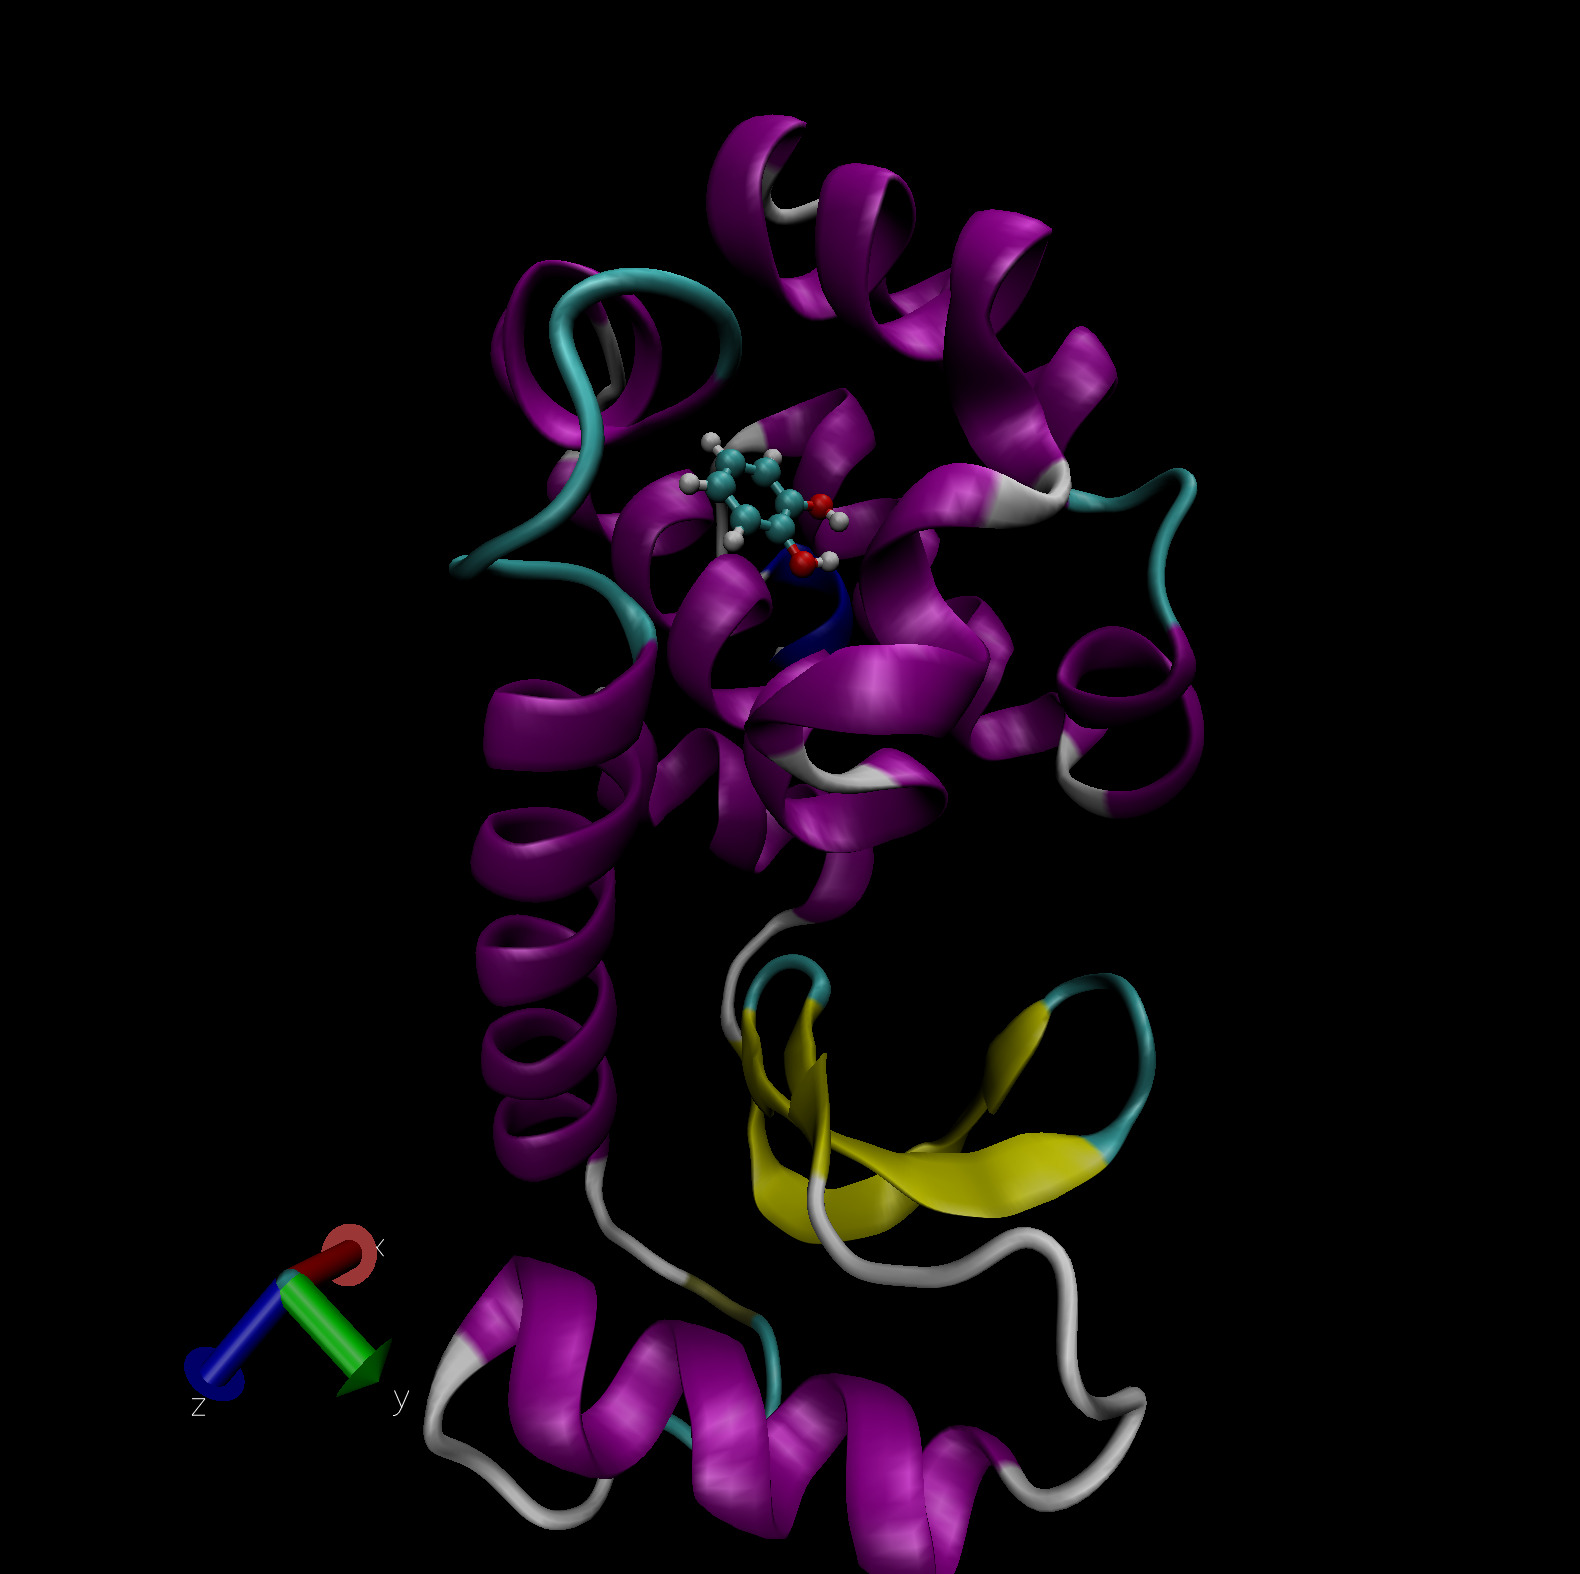
\includegraphics[width=\textwidth]{T4-Catechol.jpeg}
    \caption{Catechol bound in the buried binding site of the T4 lysozyme L99A/M102Q double mutant. Visualization in VMD.}
    \label{fig:T4}
\end{figure}

\subsection{QM-PBSA Binding Free Energies}
In this tutorial we will calculate the binding free energy of catechol to the T4 lysozyme L99A/M102Q mutant. We will employ a simplified QM-PBSA approach \cite{Fox2014,Gundelach2021} on a single snapshot of the protein-ligand complex. 

The QM-PBSA approach is a quantum-mechanical adaptation of traditional MM-PBSA, which is an end-point, implicit solvent, binding free energy method. In this approach, the binding free energy is given by
\begin{equation}
    \Delta G_{\textrm{bind}}= G_{\textrm{complex}} - G_{\textrm{host}} - G_{\textrm{ligand}},
    \label{net}
\end{equation}
where $G_{\textrm{complex}}$, $G_{\textrm{host}}$, and $G_{\textrm{ligand}}$ is the free energy of, respectively, the complex, host and ligand in an implicit solvent. Each of these can be decomposed into three terms,
\begin{equation}
    G=E + \Delta{}G_{\textrm{solv}} - TS,
    \label{energy_terms}
\end{equation}
where $E$ is the total gas-phase energy, $\Delta{}G_{\textrm{solv}}$ is the free energy of solvation and $-TS$ is an entropy correction term. In this tutorial, the entropy term will be ignored, as it is usually calculated in other programs using normal mode analysis. The linear-scaling DFT code ONETEP will be used to calculate the gas-phase and solvation free energy of the complex, host and ligand at a fully quantum-mechanical level. 

\section{Setting up the calculations}

This tutorial relies on functionality in ONETEP v6.1.3.1 or later.\\

We will set up three separate calculations, one each for the protein-ligand complex, the protein (host) and catechol (ligand). The structure of the complex was taken from a molecular dynamics simulation of the complex used in two QM-PBSA studies on this system \cite{Fox2014,Gundelach2021}. The structure of the unbound ligand and host were obtained from the complex by deletion of the respective molecules. Apart from the atomic coordinates, we must specify the details of the ONETEP single-point calculations, provide pseudopotentials for the atoms present in the system and adapt job submission scripts to run the calculations on the supercomputer of choice. 

\subsection{The input files}
The ONETEP input file, referred to as the \verb|.dat| file, contains two main elements: 1) the coordinates and atom types of the system (i.e the structural information) and 2) the details of the calculation. Due to the large system size, we have split theses two components across separate files: the \verb|.dat| file, which contains the structural information, and a \verb|.header| file which contains instructions for ONETEP. This header file is included in the \verb|.dat| file via the command \verb|includefile|. All information could also be contained in a single \verb|.dat| file; however, the use of a separate header file can make it easier to set up hundreds or even thousands of calculations which differ only in the coordinates and not the calculation settings. 

\subsubsection{\texttt{.dat}}
The two blocks included in the \verb|.dat| file are \verb|lattice_cart| and \verb|positions_abs|, which specify the simulation cell and absolute positional coordinates of each atom within the simulation cell, respectively. The \verb|includefile| command on the first line specifies the header file to include for the calculation.

\subsubsection{\texttt{.header}}
This \verb|.header| file contains all further details of the ONETEP calculation. The \verb|species| block specifies the name, element, atomic number, number of NGWFs and the NGWF radius for each atom type in the system. The \verb|species_pot| lists the names of the pseudopotential files for each atom type. The rest of the file consists of ONETEP keywords which control the details of the calculation. The provided header files are fully commented, and details on each keyword are given in the ONETEP keyword directory (\url{http://onetepkeywords.icedb.info/onetepdoc}). We will be performing single-point energy calculations using the PBE exchange-correlation functional, the D2 dispersion correction and ONETEP's minimal paramater implicit solvent model. The calculation will output verbose detail and an \verb|.xyz| file for easy visualization. The total system charge is +9 for the complex and host and 0 of the ligand. The implicit solvent is set to use the default parameters for water. 

\subsection{Submission Scripts}
Due to the large system size of over 2500 atoms, these single-point calculations can only be run on a supercomputer. Thus, a submission script appropriate for the HPC environment you are working on will be necessary. The standard distribution of ONETEP provides sample submission scripts for a variety of HPC systems. These can be found in your ONETEP directory under \verb|hpc_resources|. 

We recommend to run the complex and host calculations on multiple compute nodes, making full use of the hybrid MPI-OMP capabilities of ONETEP. On the national supercomputer ARCHER2, the use of 4 compute nodes (128 cores each) with 32 MPI processes and 16 OMP threads per process results in a wall-time of about 8 hours. Due to the much smaller size of the ligand, the calculation on the ligand in solvent should be limited to a single node, with at most 10 MPI processes. 

\section{Evaluating the Outputs}
Upon successful completion of the calculations, we will examine the three \verb|.out| files created. Each of these files contains the full details and log of the calculation, as well as the final results and some timing information. While much information about the system can be gained from the output files, we will focus first only on the final results necessary to estimate the binding free energy of the ligand, catechol, to the protein. 

\begin{table}[]
\centering
\begin{tabular}{l|d{8.0}d{8.0}d{5.2}|d{5.2}}
kcal/mol    & 
\multicolumn{1}{c}{Complex} & \multicolumn{1}{c}{Host}    & \multicolumn{1}{c|}{Ligand}  & \multicolumn{1}{c}{Complex$-$Host$-$Ligand} \\ \hline
$E$           & -7372184.3 & -7328209.2 & -43940.1 & -35.0               \\
$\Delta{}G_{\textrm{solv}}$ & -2615.0    & -2613.3      & -9.7     & 8.0                \\ \hline
$G$           & -7374799.3 & -7330822.5 & -43949.7 & -27.1              
\end{tabular}
\caption{Results (energies in kcal/mol) of complex, host and ligand single-point energy calculations for catechol bound to T4 lysozyme using ONETEP.}
\label{tab:results}
\end{table}

% OLD results
% \begin{table}[]
% \centering
% \begin{tabular}{l|lll|l}
% kcal/mol    & Complex    & Host       & Ligand   & Complex-Host-Ligand \\ \hline
% E           & -7371428.1 & -7327455.7 & -43936.5 & -35.9               \\
% G_{solv} & -2392.3    & -2393      & -8.4     & 9.1                 \\ \hline
% G           & -7373820.4 & -7329848.7 & -43944.9 & -26.8              
% \end{tabular}
% \caption{Results of complex, host and ligand single-point energy evaluation for catechol bound to T4-lysozyme using ONETEP.}
% \label{tab:results}
% \end{table}

As outlined in equations \ref{net} and \ref{energy_terms} we need to calculate the total free energy of the complex, host and ligand before subtracting the total energy of the host and ligand from that of the complex. As stated before, we will be ignoring any entropy contributions in this tutorial. The total energy is then the sum of the total gas phase energy and the solvation free energy. These energies are summarized in an easy to read section at the very end of the output files, just before the timing information. To find it, search the output file for \texttt{Total energy in solvent}. This section breaks down the different energy contributions and states the total energies in vacuum (gas phase) and in solvent as well as the solvation free energy. Table \ref{tab:results} summarizes the energy values obtained. To estimate the binding free energy we simply apply equation \ref{net} to yield:
\begin{equation}
    \Delta G_{\textrm{bind}}=G_{\textrm{complex}}-G_{\textrm{host}}-G_{\textrm{ligand}}= -7374799.3 -(-7330822.5) - (-43949.7) = -27.1 \textrm{kcal/mol}.
\end{equation}
 Thus, the estimated binding energy of catechol to the T4 lysozyme is -27.1 kcal/mol. However, there are a number of severe limitations of this estimate: 1) the entropy correction term $-TS$ has been neglected; 2) only a single snapshot was evaluated; 3) the implicit solvent model incorrectly interprets the buried cavity in the T4 lysozyme, and 4) the QM-PBSA method is designed to calculate relative binding free energies between similar sets of ligands. For an in depth look at the full application of the QM-PBSA binding free energy method to 7 ligands binding to the T4 lysozyme and a discussion of the errors, convergence and limitations of the method, please consult our recent publication \cite{Gundelach2021}.  
\subsection{Cavity Correction}
The minimal-parameter PBSA solvent-model implemented in ONETEP incorrectly handles the buried cavity in the T4 lysozyme (L99A/M102Q). This is a known issue for solvent models based on the solvent accessible surface area, and has been described in detail in 2010 by Genheden \textit{et al.} \cite{Genheden2010}, and in 2014 by Fox \textit{et al.} \cite{Fox2014}. 

In the un-complexed protein calculation, i.e the host, the surface area of the interior of the buried binding site is counted towards the solvent accessible surface area (SASA) used to calculate the non-polar solvation term. Thus, the non-polar term of just the protein is larger than that of the complex indicating the formation of a larger cavity in the solvent. Conceptually, the SASA model creates an additional, fictitious, cavity in the solvent with the SASA of the buried binding site. Because the non-polar term of both the protein and complex are known, a post-hoc cavity-correction may be applied to remove the additional (spurious) contribution of the buried cavity to the non-polar solvation energy. A full derivation is provided in \cite{Fox2014}.

\begin{equation}
    E_{\textrm{cav-cor}}=7.116(E^{\textrm{host}}_{\textrm{non-polar}}-E^{\textrm{complex}}_{\textrm{non-polar}})=7.116(289.5 - 286.2) = 23.5 \text{ kcal/mol}.
    \label{eq:cav-cor}
\end{equation}

Applying the cavity correction term calculated above to the binding free energy, we obtain a cavity-corrected binding free energy of $-27.1 + 23.5 = -3.6$ kcal/mol. For comparison, the experimental binding energy of catechol to the T4 lysozyme is -4.4 kcal/mol. It should however be noted, that the close correspondence of this single snaphot QM-PBSA binding free energy to the absolute experimental energy is likely a lucky coincidence, as the QM-PBSA method is mainly applicable to relative binding free energies and the entropy correction term has not yet been included. 

\section{Properties}
We will now show how a number of useful properties of the system can be studied through a \textit{properties calculation}. In the interest of saving computational time, and for clarity of presentation, we will use the ligand system as an example.

Add the following keywords to the \texttt{.header} file of the ligand calculation:\\

\noindent
\texttt{do\_properties T}\\
\texttt{dx\_format T}\\
\texttt{cube\_format F}\\

\noindent
and run it again. 

The first of these keywords instructs ONETEP to perform a \textit{properties calculation} towards the end of the run. This will calculate, among others, Mulliken charges on the atoms, bond lengths, the HOMO-LUMO gap, the density of states (DOS) and some grid-based quantities, such as the HOMO and LUMO canonical molecular orbitals, electronic charge density and potential. The grid-based quantities (often called \textit{scalarfields}) can be output in three different formats: \texttt{.cube}, \texttt{.dx}, and \texttt{.grd}. By default \texttt{.cube} files are written, and not the other two formats. In this example we switch off \texttt{.cube} output and turn on \texttt{.dx} output. This is effected by the last two keywords.

Once your calculation finishes, you will see that quite a number of \texttt{.dx} files have been produced:
\begin{itemize}
    \item ...\texttt{\_HOMO.dx} -- density of the canonical HOMO orbital.
    \item ...\texttt{\_LUMO.dx} -- density of the canonical LUMO orbital.
    \item ...\texttt{\_HOMO-}$n$\texttt{.dx} -- density of the $n$-th canonical orbital below HOMO.    
    \item ...\texttt{\_LUMO+}$n$\texttt{.dx} -- density of the $n$-th canonical orbital above LUMO.    
    \item ...\texttt{density.dx} -- the electronic density of the entire system.
    \item ...\texttt{potential.dx} -- the total potential (ionic + Hartree + XC) in the system.
    \item ...\texttt{electrostatic\_potential.dx} -- the electrostatic potential (ionic + Hartree) in the system.
\end{itemize}
These files correspond to the calculation in solvent. There will be a second set of \texttt{.dx} files with \texttt{vacuum} in their names -- these correspond to the calculation in vacuum. This lets you study and visualize in-vacuum and in-solvent properties separately and to perform comparisons between the two. Here, you can expect the scalarfields to be rather similar between in-vacuum and in-solvent because the ligand is charge-neutral and polarizes the solvent only very slightly. 

There is a separate tutorial (Tutorial 5) devoted to visualization. You can use the skills taught there to create fancy visualizations of the properties of your choice. Here we will only show how to produce a neat visualization of the electronic density coloured by the electrostatic potential using VMD.

Load the electronic density and the electrostatic potential into one molecule, and the atomic coordinates into a separate molecule. This will make it easier treat the scalarfields and the atomic coordinates separately. To achieve this, issue:

\begin{verbatim}
vmd ligand_2001_density.dx ligand_2001_electrostatic_potential.dx -m ligand_2001.xyz    
\end{verbatim}

Once VMD loads the files, go to \vmd{Graphics/Representations}. Ensure \vmd{Selected Molecule} (at~the top of the window) is the \texttt{.xyz} file (atomic coordinates). Under \vmd{Drawing Method} Choose \vmd{CPK} -- this will create a ball-and-stick drawing of the ligand. Switch \vmd{Selected Molecule} to the \texttt{.density.dx} file to operate on the electronic density scalarfield. Under \vmd{Drawing Method} choose \vmd{Isosurface} if it is not chosen already. Choose an \vmd{Isovalue} of \vmd{0.1} to pick a reasonable density isovalue to plot. Under \vmd{Coloring Method} choose \vmd{Volume} (you might need to scroll to the very bottom to get there). In the tiny drop-down window to the right of \vmd{Coloring Method} switch from scalarfield 0 (the density itself) to scalarfield 1 (the potential) -- this will colour the density \textit{with} the potential. For \vmd{Material} (further to the right) choose \vmd{Glass2} -- this will choose a somewhat translucent material that will let us see both the ball-and-stick model and the electronic density. Under \vmd{Draw} in the bottom-right of the window, choose \vmd{Solid Surface} instead of \vmd{Points}. Finally, let's change the range of the potential to the kinds of values that occur at the distance from the molecule at which our electronic density isosurface lies. These have been determined by trial and error. There are four tabs just above \vmd{Coloring Method}. Somewhat counterintuitively, switch to \vmd{Trajectory}, where, under \vmd{Color Scale Data Range} you can enter the minimum and maximum values for the potential (in eV). Enter \vmd{-1} in the left field and \vmd{1.5} in the right field and click \vmd{Set}. This should give a nice representation, which you can then rotate and translate to your liking using the mouse in the \vmd{OpenGL Display} window. Once you are satisfied, you can render the final image by going to \vmd{File/Render}. In the top drop-down menu choose \vmd{Tachyon} and click on \vmd{Start Rendering}. After a short while you will get a \texttt{.tga} (``TARGA format'') file in the directory you are working in. It will look more or less like the graphics in Fig.~\ref{fig:denspot}. Most graphics manipulation programs and graphics viewers read \texttt{.tga} files. If you have \texttt{ImageMagick} installed, you can use it to convert the image to a more common format, like \texttt{.png}:

\begin{verbatim}
convert vmdscene.dat.tga vmdscene.dat.png    
\end{verbatim}

\begin{figure}[hbtp]
    \centering
    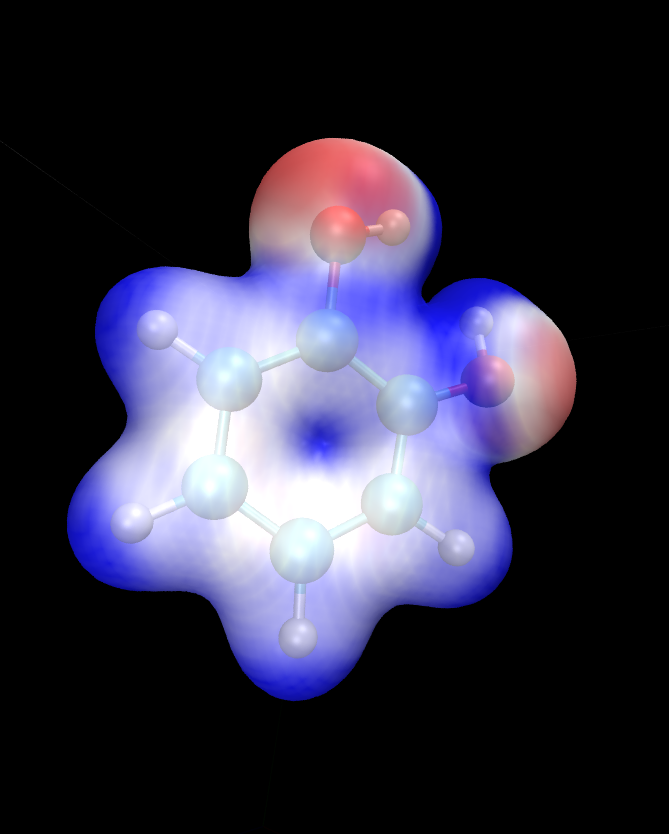
\includegraphics[width=0.5\textwidth]{vmdscene.dat.png}
    \caption{Visualization of the ligand in VMD. A ball-and-stick model of the molecule is shown, together with an isosurface of the electronic density, coloured by the electrostatic potential.}
    \label{fig:denspot}
\end{figure}

\newpage
\subsection{Atomic charges}
\subsubsection{Mulliken population analysis}
By default, during a properties calculation, ONETEP performs Mulliken population analysis, calculating partial atomic charges. The charges are written to the output file, in a table that looks like this:

%\begin{minipage}{\linewidth}
\begin{verbatim}
    Mulliken Atomic Populations
    ---------------------------
Species  Ion    Total   Charge (e)
==================================
  O      1       6.750     -0.750
  H      2       0.448      0.552
  C      3       3.817      0.183
...
==================================
\end{verbatim}
%\end{minipage}

The partial charges (in the electrons-are-negative sign convention) are output in the last column.

Mulliken population analysis has a number of drawbacks, chief among which is that it depends on the basis set used and there is no well-defined complete basis set limit. Below we discuss two alternative schemes that can be used in ONETEP: Natural Population Analysis (NPA) and Density-Derived Electrostatic and Chemical (DDEC) analysis.
\subsubsection{Natural Population Analysis}
In Natural Population Analysis the set of non-orthogonal, optimized NGWFs is transformed into a set of orthogonal atom-centered Natural Atomic Orbitals (NAOs). This approach lets empty, highly-diffuse orbitals distort to achieve orthogonality with their more highly-preserved occupied counterparts, ensuring the final
NAO population is stable with respect to basis set size. More details, and references to papers on the method, can be found in the documentation for this functionality at \url{www.onetep.org/pmwiki/uploads/Main/Documentation/nbo_onetep.pdf}.

To perform Natural Population Analysis \textit{in lieu} of Mulliken population analysis, add the following keyword to your previous ligand calculation:\\

\noindent
\texttt{write\_nbo T}\\

\noindent
and run it again. Keep the three keywords you added last time.\\[2cm]

Once your calculation completes you will find the results of NPA in your output file. They will look like this:\vspace{-0.3cm}
%\begin{minipage}{\linewidth}
\begin{verbatim}
================================================
               Natural Population               
------------------------------------------------
 Summary                                        
------------------------------------------------
   Atom        Population (e)      Charge (e)   
------------------------------------------------
 O        1         6.7313861      -0.7313861
 H        2         0.4487370       0.5512630
 C        3         3.7852506       0.2147494
...
------------------------------------------------
\end{verbatim}
%\end{minipage}

\subsubsection{Density-Derived Electrostatic and Chemical (DDEC) analysis}
ONETEP uses the DDEC3 method\cite{ddec3} to effect atoms-in-molecule electron density partitioning, producing partial charges, as well as higher multipoles (if desired), which are both chemically meaningful and give a faithful reproduction of the electrostatic potential of the QM system. More details, and references to papers on the method, can be found in the documentation at \url{www.onetep.org/pmwiki/uploads/Main/Documentation/ddec.pdf}. 

To perform DDEC analysis \textit{in lieu} of Mulliken population analysis, add the following keyword to your previous ligand calculation:\\

\noindent
\texttt{ddec\_calculate T}\\

\noindent
You will also need to add a \texttt{block ddec\_rcomp} that will specify where the reference ion densities can be found. You will need \textit{two} reference density files for every atomic species in your system -- one for the core and one for the total density, except for H and He which only require the total density file. The reference density files for a number of often-found elements can be found in the \texttt{c2\_refdens} directory of your ONETEP installation. Fortunately all the files necessary for our ligand calculation (so, reference densities for C, H and O) are already there. Add the following block to your ligand input file:

\noindent
\begin{verbatim}
%block ddec_rcomp
H ALL "H_c2.refconf"
O ALL "O_c2.refconf"
O CORE "O_c2.coreconf"
C ALL "C_c2.refconf"
C CORE "C_c2.coreconf"
%endblock ddec_rcomp
\end{verbatim}
\noindent
and copy the five files listed in the block from the \texttt{c2\_refdens} directory to where your calculation resides. The documentation explains where you can find reference density files for other elements, should you ever need them.

Once you re-run your ligand calculation, you will find the results of DDEC analysis towards the end of your output file. They will look like this:

\begin{verbatim}
------------------------------------------------
             DDEC Charges (X=0.21)              
------------------------------------------------
   Atom        Population (e)      Charge (e)   
------------------------------------------------
 O        1         8.5534066      -0.5534066
 H        2         0.5775414       0.4224586
 C        3         5.8305022       0.1694978
...
------------------------------------------------
\end{verbatim}

\subsubsection{Comparison of Mulliken, NPA and DDEC charges}
The three approaches for calculating partial charges are compared in Table~\ref{tab:charges}. Mulliken charges are, in general, the most pronounced out of the three, while DDEC partial charges are overall smaller in absolute value. The predictions of NPA are rather close to Mulliken analysis, while DDEC differs more from the first two.

\begin{table*}[htbp]
\caption{
Comparison of three approaches for calculating partial charges for the ligand.}
\centering
\begin{tabular}{|c|c|d{2.3}|d{2.3}|d{2.3}|}
\hline
{Atom number} & Species & \multicolumn{1}{c|}{Mulliken charge}&
\multicolumn{1}{c|}{NPA charge}&
\multicolumn{1}{c|}{DDEC charge}
\\ 
\hline
\hline
1 & O & -0.750 & -0.731 & -0.553\\
2 & H & 0.552 & 0.551 & 0.422 \\
3 & C & 0.183 & 0.215 & 0.169 \\
4 & C & -0.319 & -0.301 & -0.229 \\
5 & H & 0.311 & 0.251 & 0.160 \\
6 & C & -0.320 & -0.261 & -0.158 \\
7 & H & 0.295 & 0.237 & 0.130 \\
8 & C & -0.313 & -0.252 & -0.124 \\
9 & H & 0.298 & 0.241 & 0.131 \\
10 & C & -0.309 & -0.300 & -0.243 \\
11 & H & 0.296 & 0.240 & 0.146 \\
12 & C & 0.230 & 0.246 & 0.216 \\
13 & O & -0.711 & -0.685 & -0.510 \\
14 & H & 0.557 & 0.549 & 0.444 \\
\hline
\end{tabular}
\label{tab:charges}
\end{table*}

But... tables are boring. How can we visualize the charges using VMD? This is not as straightforward as we would like. The structure (atomic coordinates) is contained in the \texttt{.xyz} file, but the charges are not. Some programs can visualize a quantity added in an extra column in the \texttt{.xyz} file (which would become something like an \texttt{.xyzq} file), but not VMD, at least not easily.

Fortunately VMD can read a different format named \texttt{.vtf}, which contains both the atomic coordinates and some scalar quantity, like charge. It is easy to convert an \texttt{.xyz} file and a list of charges to a \texttt{.vtf} file. We provide a simple \texttt{bash} script with this tutorial that does exactly that. It scans a ONETEP \texttt{.out} file for charge information (be it Mulliken, NPA or DDEC charges) and extracts the values of the charges on all atoms. It then looks for a corresponding \texttt{.xyz} file and, if found, it produces a \texttt{.vtf} file ready for visualizing with VMD.

To use it, download the provided script called \texttt{out2charge}, put it in your \texttt{\$PATH}, and run it on your output:

\begin{verbatim}
out2charge ligand_2001.out    
\end{verbatim}

If everything goes well, you should see the following output:

\begin{verbatim}
Charges were output to ligand_2001.charge.
The files ligand_2001.xyz and ligand_2001.charge will be used
to construct ligand_2001.vtf.
Load ligand_2001.vtf into VMD and select 'Coloring method -> charge'.
\end{verbatim}

Indeed, a new file \texttt{ligand\_2001.charge} will be produced, containing the charges extracted from the \texttt{.out} file. These charges, together with the information in the \texttt{.xyz} file will be used to construct a \texttt{.vtf} file readable by VMD. Load this file into VMD:

\begin{verbatim}
vmd ligand_2001.vtf
\end{verbatim}

\noindent{}and go to \vmd{Graphics/Representation}. For \vmd{Drawing Method} choose \vmd{CPK} and for \vmd{Coloring Method} choose \vmd{Charge}. You will get a nice ball-and-stick model of your ligand, with the atoms coloured accorind to charge. In Fig.~\ref{fig:charges} we show a comparison of the plots for the three ways of partitioning charge that we described earlier.

\begin{figure}[htb]
    \centering
    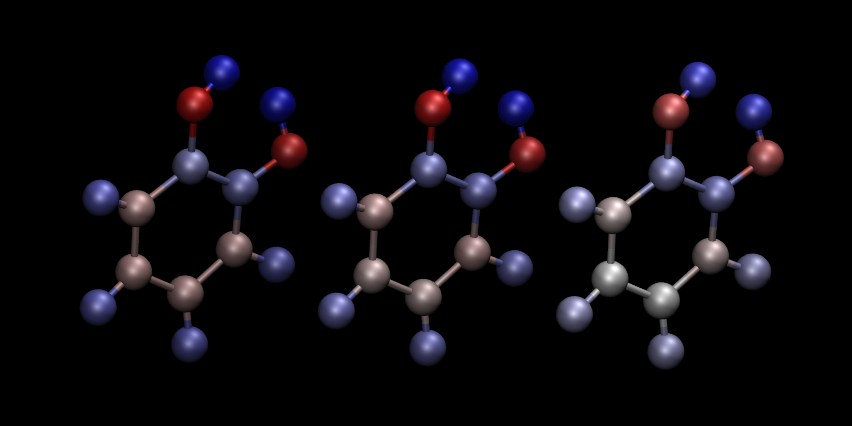
\includegraphics[width=0.8\textwidth]{vmdscene.pov.png}
    \caption{Comparison of atomic charges on the ligand: Mulliken (left), NPA (middle) and DDEC (right). Warm colours correspond to negative charges. Visualization in VMD.}
    \label{fig:charges}
\end{figure}

\newpage
\printbibliography



\end{document}